\documentclass{beamer}

\usepackage[frenchb]{babel}
\usepackage[utf8x]{luainputenc}
\usepackage{graphicx}
\usepackage{tikz}
\usetikzlibrary{graphdrawing,graphs}
\usegdlibrary{layered}

% There are many different themes available for Beamer. A comprehensive
% list with examples is given here:
% http://deic.uab.es/~iblanes/beamer_gallery/index_by_theme.html
% You can uncomment the themes below if you would like to use a different
% one:
%\usetheme{AnnArbor}
%\usetheme{Antibes}
%\usetheme{Bergen}
%\usetheme{Berkeley}
%\usetheme{Berlin}
%\usetheme{Boadilla}
%\usetheme{boxes}
%\usetheme{CambridgeUS}
%\usetheme{Copenhagen}
%\usetheme{Darmstadt}
\usetheme{default}
%\usetheme{Frankfurt}
%\usetheme{Goettingen}
%\usetheme{Hannover}
%\usetheme{Ilmenau}
%\usetheme{JuanLesPins}
%\usetheme{Luebeck}
%\usetheme{Madrid}
%\usetheme{Malmoe}
%\usetheme{Marburg}
%\usetheme{Montpellier}
%\usetheme{PaloAlto}
%\usetheme{Pittsburgh}
%\usetheme{Rochester}
%\usetheme{Singapore}
%\usetheme{Szeged}
%\usetheme{Warsaw}

\title{Jeu multi-joueurs sur les graphes d'argumentation}



% Let's get started
\begin{document}

  \begin{frame}
    \titlepage
  \end{frame}

  \begin{frame}{Présentation informelle}{graphe d'argumentation}
    \begin{center}
      \begin{tabular}{cc}
        \onslide<1->
        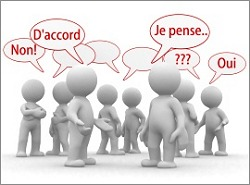
\includegraphics[scale=2]{../docs/images_presentation/discus.jpg} &
        \onslide<3->
        \begin{tikzpicture}[>=stealth]
        \graph [ layered layout, nodes = {scale=0.75, align=center} ] {
        "a1" -> "q";
        "a2" -> "a1";
        "a3" -> "a1";
        "a4" -> "a1";
        "a5" -> "a3";
        };
        \end{tikzpicture}\\
      \end{tabular}
    \end{center}

    \onslide<2->
    On a un graphe d'argumentation $F = \langle \mathcal{A}, \mathcal{R}, V \rangle$
    \begin{itemize}
      \item $\mathcal{A}$ : L'ensemble des arguments.
      \item $\mathcal{R} \subseteq \mathcal{A} \times \mathcal{A}$ : $(a,b) \in \mathcal{R}$ si $a$ "attaque" $b$.
      \item $V: \mathcal{A} \rightarrow \mathbb{N} \times \mathbb{N} : V(a) = (v^+, v^-)$ signifie que $a$ à $v^+$ "like" et $v^-$ "dislike".
    \end{itemize}
  \end{frame}

  \begin{frame}{Présentation informelle}{analyse du débat}
    \begin{center}
      
\includegraphics[scale=0.3]{../docs/images_presentation/Clipart-Meeting.jpg}
    \end{center}

    \begin{overprint}
      \onslide<1>
      \begin{itemize}
        \item Un groupe d'agents va se regrouper.
        \item Ils ont connaissance de tout le graphe d'argumentation.
        \item Chacun à un avis sur la question du débat.
        \item On matérialise cela par un vote privé sur chacun des arguments.
      \end{itemize}
      \onslide<2>
      Quelques petites définition avant de continuer.
      \begin{enumerate}
        \item La valeur d'un argument est calculée en fonction de son nombre de votes et de la valeur des arguments qui l'attaque.
        \item La valeur du graphe d'argumentation est la valeur de la question.
      \end{enumerate}

      $\rightarrow$ L'avis d'un agent est défini par la valeur de son graphe.
    \end{overprint}
  \end{frame}

  \begin{frame}{Analyse du débat}{Le jeu}
    \begin{center}
      \begin{tabular}{ccc}
        \onslide<1->
        \begin{tikzpicture}[>=stealth]
        \graph [ layered layout, nodes = {scale=0.75, align=center} ] {
        "a1\\ (0,1)" -> "q\\ (0,0)\\lm = 0.99980008";
        "a2\\ (1,0)" -> "a1\\ (0,1)";
        "a3\\ (1,0)" -> "a1\\ (0,1)";
        "a4\\ (0,1)" -> "a1\\ (0,1)";
        "a5\\ (0,0)" -> "a3\\ (1,0)";
        };
        \end{tikzpicture} &

        \begin{tikzpicture}[>=stealth]
        \graph [ layered layout, nodes = {scale=0.75, align=center} ] {
        "a1\\ (1,0)" -> "q\\ (0,0)\\lm = 0.99039208";
        "a2\\ (1,0)" -> "a1\\ (1,0)";
        "a3\\ (0,1)" -> "a1\\ (1,0)";
        "a4\\ (0,0)" -> "a1\\ (1,0)";
        "a5\\ (0,1)" -> "a3\\ (0,1)";
        };
        \end{tikzpicture} &
        \onslide<3->
        \begin{tikzpicture}[>=stealth]
        \graph [ layered layout, nodes = {scale=0.75, align=center} ] {
        "a1\\ (0,1)\\ (1,0)" -> "q\\ (0,0)\\lm = 0.98725";
        "a2\\ (1,0)\\ (0,1)" -> "a1\\ (0,1)\\ (1,0)";
        "a3\\ (1,0)\\ (1,0)" -> "a1\\ (0,1)\\ (1,0)";
        "a4\\ (1,0)\\ (0,0)" -> "a1\\ (0,1)\\ (1,0)";
        "a5\\ (0,1)\\ (1,0)" -> "a3\\ (1,0)\\ (1,0)";
        };
        \end{tikzpicture}\\
      \end{tabular}
    \end{center}
    \onslide<1->
    Avis des joueurs avec la valeur de leur graphe.
  \end{frame}

  \begin{frame}{Présentation informelle}{Le jeu}
    \begin{minipage}[c]{.30\linewidth}
      \begin{overprint}
        \onslide<1>
        \begin{tikzpicture}[>=stealth]
          \graph [ layered layout, nodes = {scale=0.75, align=center} ] {
          "a1\\ (0,0)\\ (0,0)" -> "q\\ (0,0)\\lm = 0.79297";
          "a2\\ (0,0)\\ (0,0)" -> "a1\\ (0,0)\\ (0,0)";
          "a3\\ (0,0)\\ (0,0)" -> "a1\\ (0,0)\\ (0,0)";
          "a4\\ (0,0)\\ (0,0)" -> "a1\\ (0,0)\\ (0,0)";
          "a5\\ (0,0)\\ (0,0)" -> "a3\\ (0,0)\\ (0,0)";
          };
        \end{tikzpicture}

        \onslide<2>
        \begin{tikzpicture}[>=stealth]
          \graph [ layered layout, nodes = {scale=0.75, align=center} ] {
          "a1\\ (0,1)\\ (1,0)" -> "q\\ (0,0)\\lm = 0.98725";
          "a2\\ (1,0)\\ (0,1)" -> "a1\\ (0,1)\\ (1,0)";
          "a3\\ (1,0)\\ (1,0)" -> "a1\\ (0,1)\\ (1,0)";
          "a4\\ (1,0)\\ (0,0)" -> "a1\\ (0,1)\\ (1,0)";
          "a5\\ (0,1)\\ (1,0)" -> "a3\\ (1,0)\\ (1,0)";
          };
        \end{tikzpicture}
      \end{overprint}
    \end{minipage}\hfill
    \begin{minipage}[c]{.70\linewidth}
      \begin{itemize}
        \item On commence le jeu avec le graphe sans vote.
        \item Les joueurs jouent chacun leur tour.
        \item A chaque tour ils peuvent voter pour, contre ou ne pas voter.
        \item ils ont le droit de changer d'avis.
        \item Leur objectif est que la valeur du graphe se rapproche de leur avis personnel.
        \item ils prennent toujours la meilleure décision
      \end{itemize}
    \end{minipage}
  \end{frame}

  \begin{frame}{Les questions}{Cas des arbres}
    \begin{itemize}
      \item<1-> A 1 joueur, la valeur finale du graphe est toujours égale à son avis personnel.
      \item<2-> Un joueur extrême ne peux jamais changer un de ses votes.
      \item<3-> Tout états d'équilibre est entre le min et le max.
      \item<4-> Il existe au moins 1 équilibre entre min et max.
      \item<5-> A deux joueurs, si la valeur initiale est entre min et max alors on converge vers cette valeur.
      \item<6-> Soit $d_i$ la distance à la valeur initiale pour l'agent i. Tout équilibre doit être à une distance inférieure à $d_i$ pour tout agents.
    \end{itemize}

    \begin{overprint}
      \onslide<1>
      \begin{center}
        \begin{tabular}{cc}
          \begin{tikzpicture}[>=stealth]
            \graph [ layered layout, nodes = {scale=0.60, align=center} ] {
            "a1\\ (0,1)" -> "q\\ (0,0)\\lm = 0.48491";
            "a2\\ (0,0)" -> "q\\ (0,0)\\lm = 0.48491";
            "a3\\ (0,1)" -> "q\\ (0,0)\\lm = 0.48491";
            "a4\\ (1,0)" -> "a2\\ (0,0)";
            "a5\\ (1,0)" -> "a3\\ (0,1)";
            "a6\\ (0,0)" -> "q\\ (0,0)\\lm = 0.48491";
            };
          \end{tikzpicture}&

          \begin{tikzpicture}[>=stealth]
            \graph [ layered layout, nodes = {scale=0.60, align=center} ] {
            "a1\\ (0,1)" -> "q\\ (0,0)\\lm = 0.54022";
            "a2\\ (0,0)" -> "q\\ (0,0)\\lm = 0.54022";
            "a3\\ (0,0)" -> "q\\ (0,0)\\lm = 0.54022";
            "a4\\ (0,0)" -> "a2\\ (0,0)";
            "a5\\ (0,0)" -> "a3\\ (0,0)";
            "a6\\ (0,1)" -> "q\\ (0,0)\\lm = 0.54022";
            };
          \end{tikzpicture}
        \end{tabular}
      \end{center}

      \onslide<2>
      Un joueur extrême est un joueur dont la valeur de son avis est toujours supérieure (resp. inférieure) ou égale à la valeur du graphe.

      Vrai car tous les arguments sont non ambigüs.

      \onslide<3>
      \begin{center}
        \includegraphics[scale=0.50]{/home/talkie/Documents/Stage/DebateGames/docs/examples/not_in_range_tau_1.png}
      \end{center}

      \onslide<4>
      Le min est la valeur minimum des joueurs. Le max est la valeur maximum.

      Toujours en recherche...

      \onslide<5>
      Cela parait vrai. Si la valeur du graphe est plus éloignée que la valeur initiale alors on a la possibilité de contrer un argument de son adversaire qui rapprocherai la valeur du graphe vers la valeur initiale.

      Une fois qu'on a voté sur un argument, changer d'avis ferait éloigné la valeur du graphe. Donc on s'arrête.

      \onslide<6>
      \vspace{1cm}
      Ca semble vrai pour 2 joueurs mais pas pour plus.
    \end{overprint}
  \end{frame}
\end{document}
